\documentclass{../res/univ-projet}

%Import des packages utilisés pour le document
\usepackage[utf8x]{inputenc}
\usepackage[francais]{babel}
\usepackage[T1]{fontenc}
\usepackage{lscape}
%\usepackage{array}
%\usepackage{hyperref}
%\usepackage{tabularx, longtable}
%\usepackage[table]{xcolor}
%\usepackage{fancyhdr}
%\usepackage{lastpage}

\definecolor{gris}{rgb}{0.95, 0.95, 0.95}

%Redéfinition des marges
%\addtolength{\hoffset}{-2cm}
%\addtolength{\textwidth}{4cm}
\addtolength{\topmargin}{-1cm}
\addtolength{\textheight}{1cm}
\addtolength{\headsep}{0.8cm} 
\addtolength{\footskip}{-0.2cm}


%Import page de garde et structures pour la gestion de projet
%\usepackage{structures}

%Variables
\logo{../res/logo_univ.png}
\title{Spécification Technique de Besoin}
\author{Kheireddine \bsc{Berkane}, Nasser \bsc{Adjibi}}
\projet{Compilateur LLVM}
\projdesc{Langage jouet Kawa}
\filiere{M1GIL - Conduite de Projet}
\version{0.7}
\relecteur{Pierre-Luc \bsc{BLOT}, Alexandre \bsc{PETRE}}
%\signataire{Florent \bsc{NICART}}
\date{\today}

\histentry{0.1}{04/11/2014}{Version initiale.}
\histentry{0.1.5}{18/11/2014}{Définition des cas d'utilisations et des exigences.}
\histentry{0.2}{03/12/2014}{Modifications par rapport au retour client du 25/11/2014.}
\histentry{0.3}{10/12/2014}{ \begin{itemize}
								 \item Les parties événements déclenchants ont été détaillées.
								 \item Les parties flots d'exceptions, ainsi que les conditions d’arrêts de toutes les exigences fonctionnelles ont été détaillées.
								 \item L'ajout des exigences opérationnelles d'interface.
								 \item Correction des erreurs signalées lors de la réunion client 04/12/2014.	
							 \end{itemize}	 	
								 }
\histentry{0.4}{22/12/2014}{ \begin{itemize}
\item Les parties événements déclenchants ont été modifiées et structurées sous forme d'une liste.
\item Les parties flots d'exceptions, ainsi que les conditions d’arrêts de toutes les exigences fonctionnelles ont été été modifiées et structurées sous forme d'une liste.
\item La suppression des exigences opérationnelles d'interface après une remarque faite par le prof du TP gestion de projet.
\item Changement de priorité de l'exigence fonctionnelle EF\_4 en secondaire car elle dépend de l'exigence EF\_3 qui est secondaire.
\item Correction des erreurs signalées lors du retour client par mail le 19/12/2014.	
\end{itemize}	 	
}
\histentry{0.5}{18/01/2015}{ \begin{itemize}
\item Élimination des exigences de réalisations qui correspondent aux exigences fonctionnelles afin d'éviter les redondances inutiles. 
\item La partie des exigences fonctionnelles a été détaillée ainsi que les scénarios des exceptions ont été spécifiés afin de faciliter les tests après.
\item Modifications apportées par rapport à la revue du lancement du projet 19/01/2015.
\end{itemize}
}
\histentry{0.6}{11/04/2015}{ 
\begin{itemize}
\item Élimination de l'exigence fonctionnelle EF\_3 : Compiler une application en mode partagé 
\item Élimination de l'exigence fonctionnelle EF\_4 : Compiler une bibliothèques partagée
\item Élimination de l'exigence fonctionnelle EF\_6 : Indiquer les chemins des dépendances entre le source de l'application et des modules (classe/interface) externes
\item Élimination de l'exigence de réalisation EXR\_4 : Compilation d'application partagée
\item Élimination de l'exigence de réalisation EXR\_6 : Compilation de bibliothèque partagée
\item Élimination de l'exigence de réalisation EXR\_25 : Définition d'attributs ou de variables de type \textbf{value}
\item Élimination de l'exigence de réalisation EXR\_26 : Définition méthode value
\item Élimination de l'exigence de réalisation EXR\_41 :  Gestion des exceptions
\item Changement du diagramme de cas d'utilisation après la discussion avec client afin de réduire quelques exigences fonctionnelles et de réalisation 
\end{itemize}
}

\newpage
\histentry{0.7}{15/04/2015}{ 
\begin{itemize}
\item Mettre l'exigence fonctionnelle EF\_3 : Afficher la version du compilateur en secondaire
\item Élimination de l'exigence fonctionnelle EF\_4 :Activer l'affichage en couleur
\item Élimination de l'exigence de réalisation EXR\_5 : Garbage collector
\end{itemize}
}


% -- Début du document -- %
\begin{document}

%Page de garde
\maketitle
\newpage
%La table des matières
\tableofcontents
\newpage



\section{Architecture globale}

% Présentation succinte du sujet et hyp de travail.
L'objectif de notre projet est de réaliser un compilateur à l'aide des outils LLVM (Low Level Virtual Machine) permettant de convertir un langage orienté objet ressemblant à Java (qu'on appellera \textbf{Kawa}) en langage machine. \\

Pour ce faire il faudra passer par différentes étapes d'analyse et de constructions afin d'obtenir le résultat attendu. Voici la schématisation (très simplifiée) de ces étapes.\\

\begin{figure}[h!]
\centering
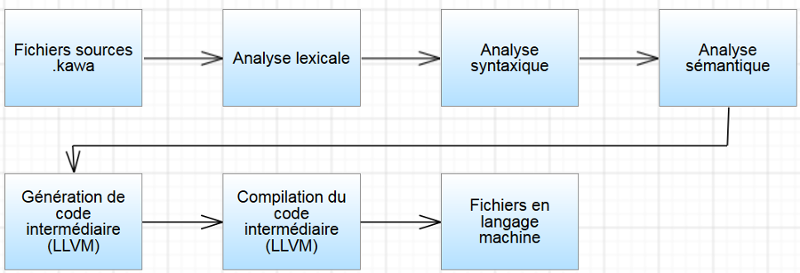
\includegraphics[scale=0.80]{archi1.png}
\caption[Schématisation de l'architectureArchitecture globale.]{Architecture globale.}
\end{figure}

Afin de comprendre et d'apréhender le travail à réaliser pour chacunes de ces étapes, nous avons mené des recherches sur le fonctionnement du compilateur ainsi que sur la plateforme LLVM. Ainsi nous proposons une architecture modulaire (reprenant les idées du schéma précédent) qui nous permet de découpler les traitements à réaliser en différentes phases d'analyses. Cela permettra également de rendre le développement du compilateur plus simple à mettre en place et la maintenance plus facile à gérer et à faire évoluer.\\

Les différents modules communiquent entre eux via des interfaces de connexion, un module orchestre les appels et l'ordre d’exécution des autres modules afin d'avoir toute la chaîne de compilation.\\

Notre architecture est donc ainsi découpée : 

 \begin{itemize}
	\item   Une structure (collection de classes) qui représente l'arbre en mémoire : le KawaTree
 	\item	Module d'analyse syntaxique (parseur)
	\item   Module d'analyse sémantique
	\item   Module back end
 \end{itemize}

\newpage

\section{Descriptions des modules}

\subsection{Le Module KawaTree}

Le KawaTree est le module au centre de la compilation car il agit comme un point de communication pour tout les autres modules. Le KawaTree est un arbre dont chacun des noeuds est une représentation des éléments du programme. Il est crée et approvisionné par le module syntaxique, lu et décoré par le module sémantique et enfin consulté par le module back end pour déterminer le code à produire.

\subsection{Module syntaxique}
C'est le module syntaxique qui débute la chaine de compilation.\\
L'objectif de cette partie est de produire un arbre syntaxique représentant le programme fourni au compilateur par le biais d'un ou de plusieurs fichiers sources Kawa.\\
C'est donc ici que la syntaxe des fichiers sources est vérifiée et validée. En cas d'erreur le compilateur doit s'arrêter et indiquer une erreur.

Le module syntaxique se découpe en deux phases : 
\begin{itemize}
	\item Analyse Lexicale : identifie et repère les \textbf{tokens} au sein des fichiers sources. 
	\item Analyse Syntaxique : identifie les chaines de caractères appartenant à la syntaxe du langage Kawa, grâce aux tokens précédements trouvées par l'analyse lexicale, afin de construire en mémoire un arbre syntaxique (AST) représentant le programme.
\end{itemize}
Remarque : ces deux phases sont cependant réalisées de manières conjointes.

\subsection{Module sémantique}
Le module sémantique est la deuxième roue de la chaine de compilation, il ne sera effectué que si le module syntaxique ne rencontre pas d'erreur.\\

Dans cette partie on vérifie la sémantique du programme et on décore (i.e. : on ajoute des informations) l'arbre fourni par le module syntaxique.\\

Il faudra donc parcourir l'AST afin de vérifier le respect des nombreuses règles sémantiques mais également afin d'y ajouter des informations nécessaires à la génération du code (module suivant).

\subsection{Module back end}
C'est la dernière étape de la chaine de compilation.
Il est chargé de traduire la structure de l'AST décoré en un language compréhensible par la machine.
Son rôle se déroule en deux étapes. La premiere étape consiste à la production du code intermédiare LLVM. La deuxieme étape quant à elle compilera le code intermédiare en code machine au format ELF.


\begin{landscape}

\section{Résumé des étapes de compilation}
\centering

\begin{figure}[h!]
\centering
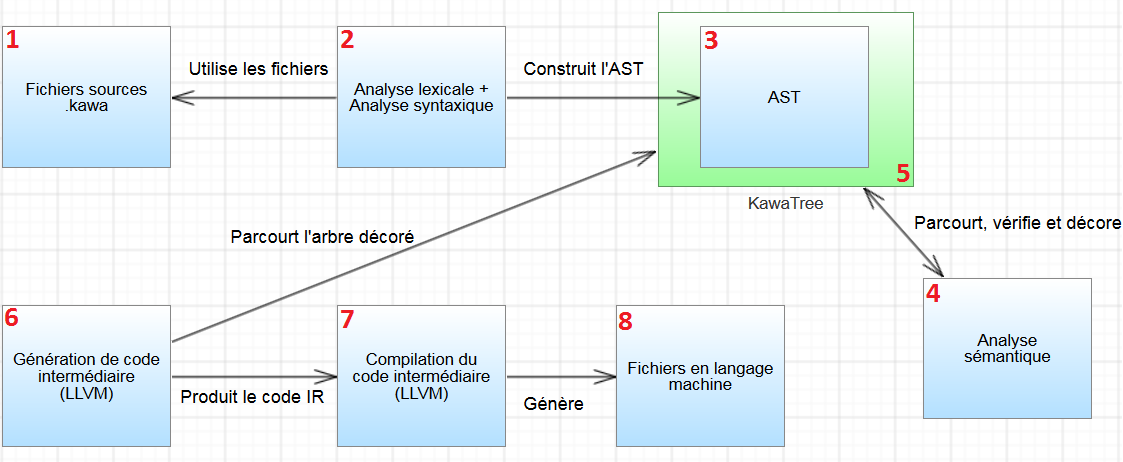
\includegraphics[scale=0.80]{archi2.png}
\caption[Architecture globale.]{Architecture globale.}
\end{figure}

\end{landscape}

\end{document}

